%TODO:
% Introduction to data collection, data processing and closing the sensing loop


\section{Data Collection}
% TODO: 
% Apply definitions
% Little introduction
% Tactics:
%    - Part into intervals
%    - Sampling rate
%    - Combinations of sensors (location/gps + 
%      accelerometer + gyroscope)
% Relate to articles
% Relate to app
% Reflect and discuss

Bikebus data collection from continuous sensing consists of: 
\begin{itemize}
    \item Location data - GPS sensor (Fine Location)
    \item Activity Recognition data from Google API - Low-power Sensors\footnote{\url{https://developers.google.com/android/reference/com/google/android/gms/location/ActivityRecognitionClient}}
\end{itemize}

Location data uses the \textit{FINE LOCATION} sensor to determine the actual path of the bike route when a bikebus has startet. To determine when a bikebus has startet and ended the notion of "Geofencing" is used to trigger when the user is inside a radius of <<INSERT RADIUS>>. 
When a geofence event has been raised some constraints must be fulfilled before the continuous data collection can begin.
\begin{itemize}
    \item The current timestamp must be within the time window <<INSERT TIME WINDOW>> of an enlisted bikebus
    \item The current activity must be of type "\textit{ON\_BICYCLE}"
\end{itemize}
Once the constraints have been fulfilled the data collection begins <<INSERT SENSING TACTIC>> by collecting locations at the sample rate of <<INSERT SAMPLE RATE>>. This is fairly expensive sensor collection because the \textit{FINE\_LOCATION} sensor is used to give street-specific accuracy of the location data. This expensive sensing operation can be improved by decreasing the sample rate (<<SPECIFY EXACTLY WHICH TACTICS THIS IS>>) and afterwards apply some filtering techniques to smooth out the path.

Along with the location data the data collection also includes Activity Recognition for assuring all collected data only is collected while biking. This eliminates the situations where stopping for a red light is accounted for in the data collection and therefore will influence the overall statistics. This combination of location and activity data will provide more accurate biking statistics. 
The activity recognition only uses the sensors defined as "Low-power".
According to the Android documentation of "Low-power sensors"\footnote{\url{https://source.android.com/devices/sensors/power-use#low_power_sensors}} the following sensors can be utilized:
\begin{itemize}
    \item Geomagnetic rotation vector
    \item Significant motion
    \item Step counter
    \item Step detector
    \item Tilt detector
\end{itemize}
The use of only "Low-power sensors" makes the activity recognition relatively energy efficient opposed to the location data.

Once the end geofence event arises the data collection can stop and the final statistics will be processed. Due to the incident of the end geofence never being triggered due to inaccurate location sensing, the program automatically stops the data collection if the current time exceeds a given time threshold <<INSERT TIME THRESHOLD>> defined from the suggested time duration of the current bikebus.

\section{Data Processing}
% TODO:
% Apply definitions
% Little introduction
% Explain Types of processing
%    - online/offline processing
%    - realtime/batch processing
% Explain processing math
%    - classification (basic)
%    - filtering algorithms
%    - compression algorithms (Trajection)
% Relate to articles
% Relate to app
% Reflect and discuss

When working with location based data one needs to take into account the amount of data which need to be processed and stored. Figure \ref{fig:system_model_for_locations_based_services} from \cite{Lee2011} shows how moving objects gathers data and sends it to mobile object databases. The location server will then be able to serve different kinds of locations based application. The leads to how Bikebus can be designed only to store the most valuable data without losing precision of data. Bikebus has cases were it could be beneficial to visualize route data or do statistical calculation on the route data.   

\begin{figure}[H]
\centering
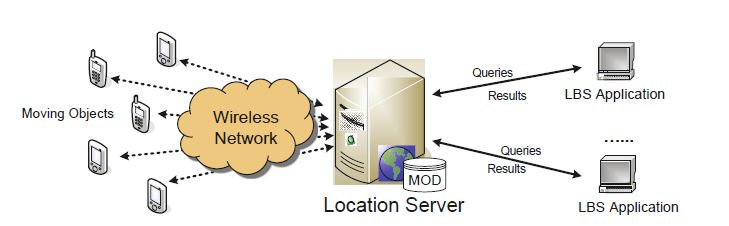
\includegraphics[scale=0.6]{LocationServer.JPG}

\caption{System model for locations based services}
\label{fig:system_model_for_locations_based_services}
\end{figure}


There are several options presented by \cite{Lee2011} how one can do data reduction and filtering techniques on spatial trajectories and thereby reduce the amount of data saved. There is batch compression (offline) and online algorithms for data reduction. Batch compression do computation on a full set of location points and then transmits it to the location server. Online algorithms computes directly on online selective data. In bikebus currently the following processing are implemented:
\begin{itemize}
    \item Douglas-Peucker compression algorithm
    \item Sliding Window compression algorithm
\end{itemize}

\begin{figure}[H]
\centering
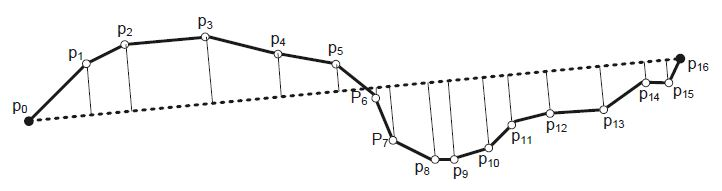
\includegraphics[scale=0.6]{DP.JPG}

\caption{Douglas-Peucker algorithm}
\label{fig:douglas_peucker_algorithm}
\end{figure}



\begin{figure}[H]
\centering
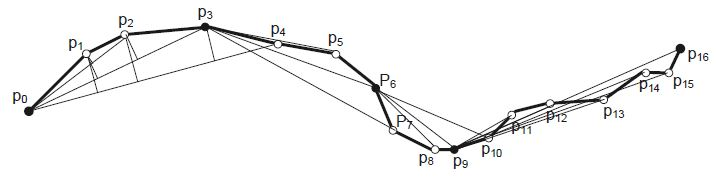
\includegraphics[scale=0.6]{SlidingWindow.JPG}

\caption{Sliding Window algorithm}
\label{fig:sliding_window_algorithm}
\end{figure}


Suggestions for further processing:
\begin{itemize}
    \item Median filtering
    \item Advanced statistics calculations (analyse per interval)
    \item Algorithm to balance the trade-off between processing space and time (Appendix \ref{app:processing_algorithm})
\end{itemize}


\section{Closing the Sensing Loop}
% TODO:
% Apply definitions
% Little introduction
% Explain concepts
%    - Sharing
%    - Privacy 
%    - Personalization
% Relate to articles
% Relate to app: 
%    - privacy: delete raw data after processing
% Reflect and discuss